\documentclass[border=8pt]{standalone}
\usepackage[T1]{fontenc}\usepackage[utf8]{inputenc}
\usepackage{helvet}\renewcommand{\familydefault}{\sfdefault}
\usepackage{tikz,xcolor}
\usetikzlibrary{arrows.meta,positioning,shapes.geometric,shapes.multipart,calc,fit,backgrounds,decorations.markings}
\definecolor{ink}{HTML}{1E1B16}\definecolor{paper}{HTML}{FBF8F2}\definecolor{clay}{HTML}{B5482A}\definecolor{soft}{HTML}{F1E9DA}\definecolor{pine}{HTML}{24402F}
\tikzset{
  every node/.style={font=\small,text=ink},
  >=Stealth, line/.style={draw=ink,line width=0.8pt},
  cls/.style={rectangle split,rectangle split parts=3,draw=ink,line width=0.8pt,fill=soft,align=left,inner xsep=6pt,inner ysep=4pt,
              rectangle split part align={center,left,left},minimum width=3.0cm},
  cls2/.style={rectangle split,rectangle split parts=2,draw=ink,line width=0.8pt,fill=soft,align=left,inner xsep=6pt,inner ysep=4pt,
              rectangle split part align={center,left},minimum width=3.0cm},
  box/.style={rectangle,draw=ink,line width=0.8pt,fill=soft,align=center,inner sep=5pt,minimum height=0.8cm},
  state/.style={rectangle,rounded corners=8pt,draw=ink,line width=0.8pt,fill=soft,align=center,inner sep=6pt,minimum width=2.2cm,minimum height=0.9cm},
  act/.style={rectangle,rounded corners=10pt,draw=ink,line width=0.8pt,fill=soft,align=center,inner sep=5pt,minimum width=2.4cm,minimum height=0.8cm},
  dec/.style={diamond,draw=ink,line width=0.8pt,fill=soft,inner sep=1pt,minimum width=0.9cm,minimum height=0.9cm},
  uc/.style={ellipse,draw=ink,line width=0.8pt,fill=soft,align=center,inner sep=3pt,minimum width=3.2cm,minimum height=1.0cm},
  note/.style={rectangle,draw=ink,line width=0.6pt,fill=yellow!12,align=left,inner sep=4pt,font=\footnotesize},
  lab/.style={font=\footnotesize,fill=paper,inner sep=1.5pt},
  err/.style={},
}
\newcommand{\actor}[3]{% x,y,label
  \draw[line width=0.8pt] (#1,#2+0.55) circle (0.17);
  \draw[line width=0.8pt] (#1,#2+0.38)--(#1,#2-0.15) (#1-0.3,#2+0.22)--(#1+0.3,#2+0.22) (#1,#2-0.15)--(#1-0.25,#2-0.6) (#1,#2-0.15)--(#1+0.25,#2-0.6);
  \node[font=\small] at (#1,#2-0.9) {#3};}
\begin{document}
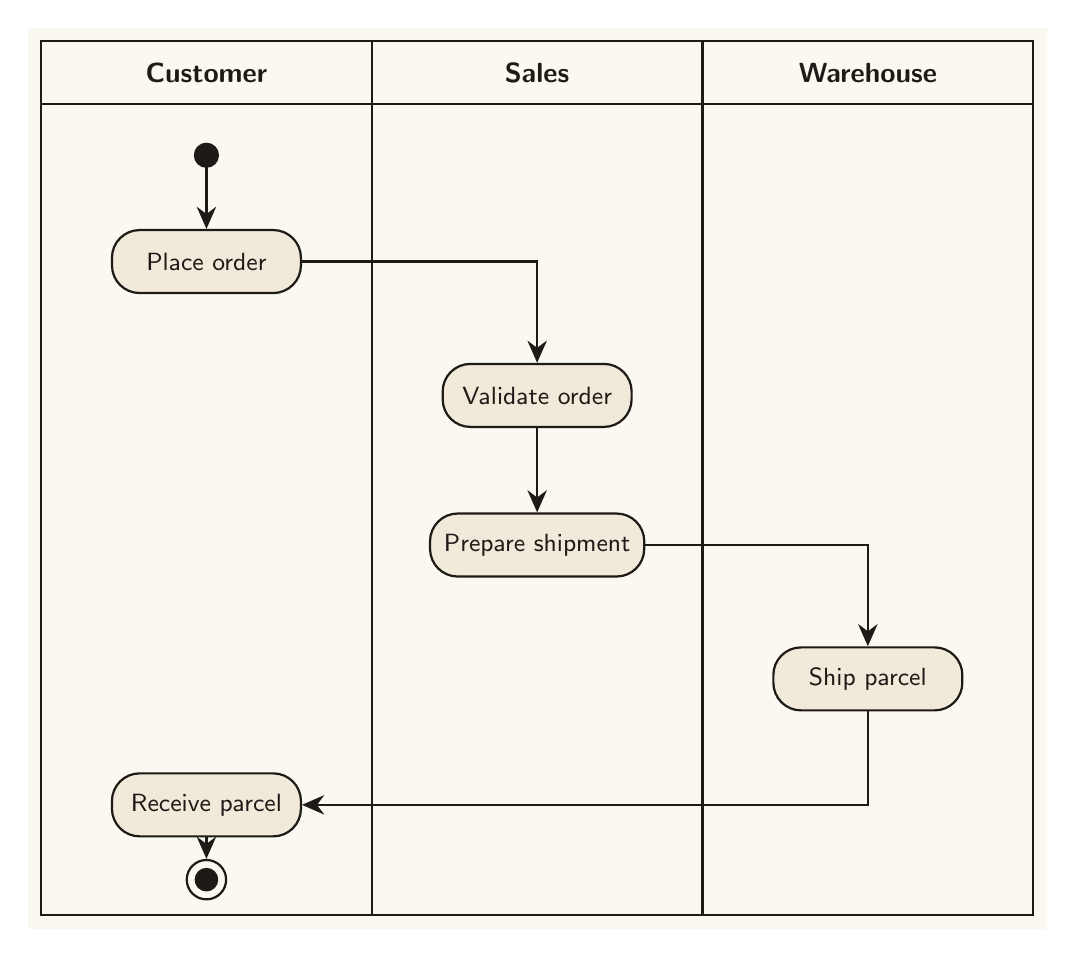
\begin{tikzpicture}[background rectangle/.style={fill=paper},show background rectangle]
\draw[line] (0,0.9) rectangle (4.2,-10.2);
\node[font=\bfseries] at (2.1,0.5) {Customer};
\draw[line] (4.2,0.9) rectangle (8.4,-10.2);
\node[font=\bfseries] at (6.300000000000001,0.5) {Sales};
\draw[line] (8.4,0.9) rectangle (12.6,-10.2);
\node[font=\bfseries] at (10.5,0.5) {Warehouse};
\draw[line] (0,0.1)--(12.6,0.1);
\fill[ink] (2.1,-0.55) circle (0.16);
\node[act] (a1) at (2.1,-1.9) {Place order};
\node[act] (a2) at (6.3,-3.6) {Validate order};
\node[act] (a3) at (6.3,-5.5) {Prepare shipment};
\node[act] (a4) at (10.5,-7.2) {Ship parcel};
\node[act] (a5) at (2.1,-8.8) {Receive parcel};
\node[circle,draw=ink,line width=0.8pt,minimum size=0.5cm] (fi) at (2.1,-9.75) {};\fill[ink] (fi) circle (0.15);
\draw[line,-{Stealth[length=8pt,width=7pt]}] (2.1,-0.7)--(a1.north);
\draw[line,-{Stealth[length=8pt,width=7pt]}] (a1.east)-|(a2.north);
\draw[line,-{Stealth[length=8pt,width=7pt]}] (a2.south)--(a3.north);
\draw[line,-{Stealth[length=8pt,width=7pt]}] (a3.east)-|(a4.north);
\draw[line,-{Stealth[length=8pt,width=7pt]}] (a4.south)|-(a5.east);
\draw[line,-{Stealth[length=8pt,width=7pt]}] (a5.south)--(fi.north);
\end{tikzpicture}
\end{document}
